%\title{emnlp 2017 instructions}
% File emnlp2017.tex
%
\PassOptionsToPackage{dvipdfmx}{graphicx} %or dvipdfm depending on the tex system

\documentclass[11pt,letterpaper]{article}
\usepackage{emnlp2017}
\usepackage{times}
\usepackage{latexsym}

\usepackage{graphicx}
\usepackage{amsmath}
\usepackage{amssymb}
%\usepackage[breaklinks=true,bookmarks=false]{hyperref}

% ==============CUSTOM PACKAGES (installed by Gota) ===================
% ref: https://github.com/jluttine/tikz-bayesnet
%\usepackage{tikz}
%\usetikzlibrary{bayesnet}
% ref: http://www.tapdancinggoats.com/latex-vector-notation.htm
\renewcommand{\vec}[1]{\mathbf{#1}}
%\usepackage{widetext}
\usepackage{array}
\usepackage{multirow}
\usepackage{longtable}
\usepackage{supertabular,booktabs}
\usepackage{tabularx}
\usepackage{tabulary}
\usepackage{xcolor}

\definecolor{_green}{rgb}{0.2745, 0.6235, 0.6157}
%\definecolor{_red}{rgb}{170,55,66}
\definecolor{_red}{rgb}{ 0.6667, 0.2157, 0.2588 }
\definecolor{test}{rgb}{ 0.6667, 0.2157, 0.2588 }
% ================================================================

% Uncomment this line for the final submission:
\emnlpfinalcopy

%  Enter the EMNLP Paper ID here:
\def\emnlppaperid{***}

% To expand the titlebox for more authors, uncomment
% below and set accordingly.
% \addtolength\titlebox{.5in}    

\newcommand\BibTeX{B{\sc ib}\TeX}


\title{Automatically Solving Word Algebra Problems with Structured Prediction Energy Networks}

% Author information can be set in various styles:
% For several authors from the same institution:
% \author{Author 1 \and ... \and Author n \\
%         Address line \\ ... \\ Address line}
% if the names do not fit well on one line use
%         Author 1 \\ {\bf Author 2} \\ ... \\ {\bf Author n} \\
% For authors from different institutions:
% \author{Author 1 \\ Address line \\  ... \\ Address line
%         \And  ... \And
%         Author n \\ Address line \\ ... \\ Address line}
% To start a seperate ``row'' of authors use \AND, as in
% \author{Author 1 \\ Address line \\  ... \\ Address line
%         \AND
%         Author 2 \\ Address line \\ ... \\ Address line \And
%         Author 3 \\ Address line \\ ... \\ Address line}
% If the title and author information does not fit in the area allocated,
% place \setlength\titlebox{<new height>} right after
% at the top, where <new height> can be something larger than 2.25in
\author{Arpit Jain\\ {\tt jain@umass.edu }  \And Gota Gando\\ {\tt ggando@umass.edu } \AND Krishna Prasad Sankaranarayanan\\ {\tt ksankaranara@umass.edu }  \And Nikhil Yadav\\
  {\tt nikhilyadav@umass.edu }}

\date{02/23/2018}

\begin{document}

\maketitle


\if0
\begin{abstract}
Solving word albegra problems automatically is a long-standing task in natural language processing (NLP). We propose a new approach for this task with structured prediction energy networks (SPENs). Our model reasons hierarchical structures of the output equations with energy functions that are parameterized by neural networks. The learning algorithm uses varied supervision, including either full equations or just the final answers. We evaluate performance
\end{abstract}
\fi

\section{Overview}
Solving word albegra problems automatically is a long-standing task in natural language processing (NLP). We plan to propose a new approach for solving algebra word problems automatically. In this task, the system needs to find a transformation from the given word problem into a set of equations which correctly represents the input word problem. To tackle this task, we apply structured prediction energy networks (SPENs), which is an energy based model where we can inject the structure knowledge of the task. We plan to start off from a simple feed-forward baseline model, and then evaluate and explore the possibilities of the SPEN model.
%%%
%%%
\section{Introduction}
Algebra word problems in general describe some particular world situation and pose a question about it. In this project, we only consider the problems where we can use a system of equations to solve the questions. Figure \ref{algebra-example} shows one example of such problems. In this case, we can express the problem as a set of algebraic equations that descrbe the mathematical relationship of entities in the problem: for example $m = 4 \times n$ and $m-4 = 6 \times (n-4)$ where $m$ and $n$ represent the age of Maria and Kate, respectively. To answer the question, we need to solve these equations and get the solution. However, we focus on finding a mapping from the word problem into an equation system in this project, as there are many automated solvers for this process.
\begin{figure}[ht]
	\centering
	Maria is now four times as old as Kate.\\
Four years ago, Maria was six times as\\
old as Kate. Find their ages now.\\
    \label{algebra-example}
\end{figure}
\subsection{Structured Prediction}
If we consider each character of the output equations as a random variable, then this task can be considered as a structured prediction task, as every output random variable would be dependent on some other variables. Furthermore, as both the input and output are sequences, we can also interpret this task as a sequence-to-sequnce task.

In many machine learning tasks, we try to predict $\textbf{y}$ given an input $\textbf{x}$. In some cases it is sufficient to use a discriminative function $F$ to predict the output such as $\textbf{y} = F( \textbf{x} )$. However, this model fails to model the structure of the output and the interactions among output components and may perform poor on more complex tasks. We can instead use \textit{an energy function} $E$ that both depends on $\textbf{x}$ and $\textbf{y}$ to model such structure and seek the optimal $\textbf{y}$ that minimizes the energy:
\begin{equation}
\hat{\mathbf{y}} = argmin_{\mathbf{y}} E( \mathbf{y}, \mathbf{x} )%E_{\mathbf{x}} (\mathbf{y})
\label{ebm0}
\end{equation}
Energy function can be seen as a scoring function that returns how compatible $\mathbf{x}$ and $\mathbf{y}$ are, or how likely they occur together.
One thing we need to note here is that there is no guarantee of the returning value of energy functions will be in the range of $\{ 0, 1\}$. One common way to address this problem and calibrate the energy is putting it through the Gibbs distribution.
\begin{equation}
P(Y|X) = \frac{ \exp{- \beta E(Y, X)} }{\int_{y \in \mathcal(Y)} \exp{- \beta E(y, X)}  }
\label{ebm1}
\end{equation}
However, it should be noted that this transformation is only possible when computing the integral term $\int_{y \in \mathcal(Y)} \exp{- \beta E(y, X)}$ is tractable.
%%%
%%%
\section{Related Works}
% TODO: COMPLETE THIS SECTION 
Solving word albegra problems automatically is a long-standing task in natural language processing (NLP). ...
%%%
%%%
\section{Problem Definition}
Following \cite{Kushman2014LearningTA}, we define a transformation of word problems to equations as a two step process. First, a template is selected to define the structure of the target equation system. Second, the selected template is instantiated with actual texts for unknowns and values for coefficients. Figure \ref{template} shows an example of template selection and instantiation. Each template has $u$ slots that represent unknown variables, and $n$ slots for coefficients of unknowns.
\begin{figure*}[ht]
	\centering
	%\includegraphics[bb=0 0 912 419, natheight=5cm]{figs/fig_encdec.pdf}%scale=0.8, 
	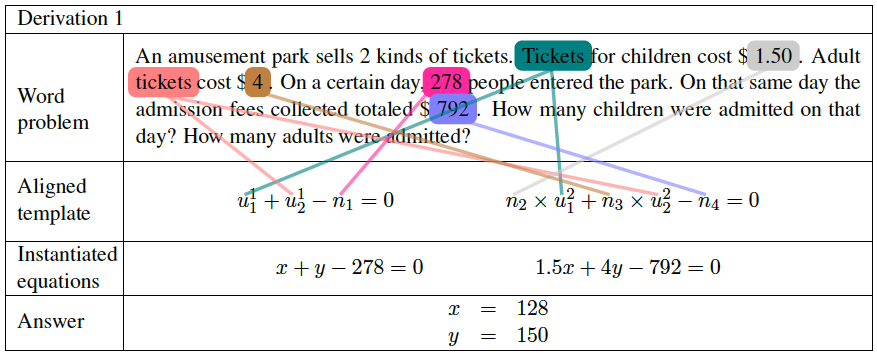
\includegraphics[bb=0 0 877 353, scale=0.5]{template.png}%scale=0.8, 
    \caption{The structure of the baseline model. Cited from \cite{Kushman2014LearningTA}}
    \label{template}
\end{figure*}
\subsection{Derivation}
In this section, we review the formulation described in \cite{Kushman2014LearningTA} and \cite{UpChChYi16}. We denote the input word problem as $\textbf{x}$, and the output as $\textbf{y}$. We call the output as a derivation, which consists of a template $T$ and an alignment $A$. Therefore we can express the output as $\textbf{y} = (T, A)$. More specifically, template $T$ is a set of equations $= \{t_0, ..., t_l\}$, and an alignment $A$ is defined as a set of pairs $(w, s)$, where where $w$ is a token in $\textbf{x}$ and $s$ is a slot instance in $T$.
%%%
%%%
\section{Approach}
\subsection{Baseline model}
We plan to use two baseline models. One is a regular feed-forward neural network that predicts the output equations directly from the input, interpreting the task as a black-box sequence-to-sequence task. Another baseline is also a neural network that jointly predicts derivation of templates and its alignments. In both cases, first the input text problem is put through a word embedding layer and a vector is assigned to each word. The first baseline then predicts the output directly after forwarding through several intermediate layers. The second baseline model on the other hand, tries to predict the template structure and its alignments at the same time. This is performed by constructing a derivation vector where the first element denotes the index of the predicted template and the other elements denote the textual or integer values of each unknowns / coefficients in the selected template.
% TODO: ADD DENSE VECTOR EXPLANATION HERE
\subsection{SPEN}
%Unlike feed-forward approaches, 
%As with other EBMs, SPEN tries to predict $y$
Structured Prediction Energy Networks (SPENs) \cite{DBLP:journals/corr/BelangerM15}\cite{DBLP:conf/icml/BelangerYM17} are one of the energy-based models (EBMs) that performs structured prediction, such as conditional random fields (CRFs), structured perceptrons, and structured SVMs (SSVMs).
There are two main differences betwen SPEN and other enegy-based models. First, SPENs can learn non-linear energy functions, as it is parameterized by a deep neural network. Similar to other EBMs, SPEN also tries to predict $y$ that minimizes the energy function. The different point is that while EBMs listed above usually assume a restricted graphical structure such as a chain or a tree and consider a linear energy function, SPEN instead considers a general energy function and assumes the non-convexity. Then, it approximates the optimal $\mathbf{y}$ with gradient descent:
\begin{equation}
\mathbf{\bar{y}} = argmin_{\mathbf{\bar{y}}} E( \mathbf{\bar{y}}, \mathbf{x} )
%Ex(y) subject to y \in \{0, 1\}
\end{equation}
\begin{equation}
\mathbf{y}^{t+1} = \mathbf{y}^t - \eta \frac{ \partial E }{ \partial \mathbf{y^t}}
\end{equation}
Additionally, SPENs are much more efficient at the inferene stage where the model predicts a candidate output $\bar{\mathbf{y}}$, as SPENs use gradient descent to approximate an optimal $\bar{\mathbf{y}}$ instead of using computationally expensive searching methods such as viterbi algorithm or beam search.
%%
\subsection{Architecture of SPEN}
Although SPEN can take general energy functions, in this work we consider the energy function consists of the global energy and the sum of local energies as follows:
\begin{align}
E_x^{local}(\bar{y}) = \sum^L_{i=1} \bar{y_i} b_i^T F(x) \\
E_x^{global}(\bar{y}) = c_2^T g(C_1 \bar{y})
\end{align}
where $g$ is a non-linearity function, each $b_i$ is a vector of parameters for each label, and the product $C_1 \bar{y}$ is a set of learned affine (linear + bias)
measurements of the output.

We give the same representation of $y$ as described in the baseline section to this energy network.
% TODO: ADD MORE DETAILED EXPLANATION WITH EQUATIONS
%%%
%%%
\section{Evaluation}
Following the existing works, we evaluate the model's performance with the overall accuracy on the ALG-514 and DRAW datasets. The predicted equation system is marked as correct if all the characters of the output exactly matches the ground truth equations. We also plan to evaluate the accuracy on several subsets of word problems to further analyze problems the model can perform well.
%%%
%%%
\section{Datasets}
We plan to use two datasets; the ALG-514 dataset proposed by \cite{Kushman2014LearningTA} which contains 514 word problems, and the DRAW dataset provided by Microsoft that contains about 1000 independent examples. One issue we are currently aware of these datasets is that ,while they include template structure of output equations for each problem, they do not provide the mapping of unknowns to text values. We plan to manually annotate such alignment information on these datasets so that we can fully make use of the template structure and its alignments.
%%%
%%%
\section{Scope}
Although it might be interesting to explore how we can improve the model itself, we limit the scope of this project to applying and evaluating the baseline MLP and SPEN model. Application of the SPEN includes designing structured representation of the output variable $y$. We are also planning to utilize the "implicit" data samples described in \cite{UpChChYi16}, which only contain the solutions of equations and not equation themselves if we have time after evaluating the baselines and the SPEN model. In this approach, we hope to jointly learn from data samples with equation labels and without such labels.
%
\nocite{*}
\bibliography{696ds_bib}
\bibliographystyle{emnlp_natbib}

\end{document}
